\documentclass[11pt,a4paper]{article}

% --- Packages ---
\usepackage[T1]{fontenc}
\usepackage[utf8]{inputenc}
\usepackage{lmodern}
\usepackage[margin=2.5cm]{geometry}
\usepackage{amsmath, amssymb, amsthm}
\usepackage{physics}
\usepackage{braket}
\usepackage{algorithm}
\usepackage{algpseudocode}
\usepackage{listings}
\usepackage{xcolor}
\usepackage{graphicx}
\usepackage{caption}
\usepackage{hyperref}
\usepackage{bookmark}
\usepackage{microtype}
\usepackage{booktabs}
\usepackage{enumitem}
\usepackage{fancyhdr}
\usepackage{titlesec}
\usepackage[style=authoryear]{biblatex}
\addbibresource{references.bib}



% --- Page style ---
\pagestyle{fancy}
\fancyhf{}
\rhead{\small Quantum Information Assignment}
\cfoot{\thepage}
\renewcommand{\headrulewidth}{0.4pt}
\setlength{\parindent}{0pt}
% --- Section formatting ---
\titleformat{\section}{\large\bfseries}{}{0em}{}[\titlerule]
\titleformat{\subsection}{\normalsize\bfseries\itshape}{}{0em}{}
\titlespacing*{\section}{0pt}{12pt}{6pt}
\titlespacing*{\subsection}{0pt}{8pt}{4pt}

% --- Code style ---
\lstdefinestyle{python}{
    language=Python,
    basicstyle=\ttfamily\small,
    keywordstyle=\color{blue!70!black}\bfseries,
    commentstyle=\color{gray},
    stringstyle=\color{orange!80!black},
    showstringspaces=false,
    breaklines=true,
    frame=single,
    rulecolor=\color{gray!40},
    backgroundcolor=\color{gray!5},
    numbers=left,
    numberstyle=\tiny\color{gray},
    numbersep=6pt,
}

% --- Hyperref ---
\hypersetup{
    colorlinks=true,
    linkcolor=blue!60!black,
    urlcolor=blue!60!black,
    citecolor=blue!60!black,
}

% --- Custom commands ---
\newcommand{\N}{\mathbb{N}}
\newcommand{\bN}{\mathbf{N}}
\newcommand{\code}[1]{\texttt{#1}}
\newcommand{\reg}[1]{\texttt{#1}}

% ================================================================
\begin{document}
% ================================================================

% --- Title ---
\begin{center}
    {\LARGE\bfseries Quantum Information Report}\\[0.3em]
    {\large Francesca Pagano}\\[0.3em]
\end{center}
\vspace{0.2em}

% ================================================================
\section{Shor's Algorithm}
% ================================================================

Shor's algorithm is a quantum algorithm for integer factorization. This problem has many implications, one of the most famous one is 
in cryptography, in particular for the RSA scheme, used in online transactions.
The fastest classical algorithm for factorization runs in sub-exponential time $e^{\mathcal{O}(n^{1/3}(\log n)^{2/3})}$.
 Instead, Shor's quantum algorithm achieves
polynomial time $\mathcal{O}(n^3)$, where $n = \lceil \log_2 N \rceil$ is the number of bits of $N$.

The speedup is obtained thanks to quantum computations based on \textit{quantum phase estimation}. 
The algorithm exists also thanks to classical results that enable the reduction of integer factorization to phase estimation and the subsequent extraction of the factors from the measured phase.

\section{1. Classical Reduction}

If $N$ is the odd composite number we want to factorize, one should then pick an integer $a$ such that $1 < a < N$ and
$\gcd(a,N)=1$. 
We define \textbf{order} of $a$ modulo $N$ the smallest positive integer $r$
such that $a^r \equiv 1 \pmod{N}$, or, equivalently, we can define $r$ as the period of the function
$f(x) = a^x \bmod N$. If $r$ is even and $a^{r/2} \not\equiv -1 \pmod{N}$, then from 
$a^r \equiv 1 \pmod{N}$ one obtains 
\begin{equation}
    \left(a^{r/2}-1\right)\!\left(a^{r/2}+1\right) \equiv 0 \pmod{N},
    \label{eq:factor}
\end{equation}
and the prime factors can be recovered via $\gcd(a^{r/2} \pm 1,\, N)$.
%The probability that a randomly chosen $a$ satisfies the conditions is at least $1/2$ when
%$N$ has two or more distinct odd prime factors, so the algorithm succeeds in $\mathcal{O}(1)$
%expected repetitions. 

Another classical aspect concerns the quantum order-finding subroutine measurement: we 
need to convert the measured phase $\varphi$ into the order $r$.
If $\varphi = m/2^{n_x}$,
one computes the continued fraction expansion of $\varphi$ and tests candidate denominators
$q$ until $a^q \equiv 1 \pmod{N}$.

% The complete procedure is summarised below.
% \begin{algorithm}[H]
% \caption{Factoring $N$ (Shor: classical steps + quantum order finding)}
% \begin{algorithmic}[1]
% \Require $N$ odd and not a prime power
% \Ensure Two nontrivial factors of $N$
% \While{true}
%     \State Pick random integer $a$ with $1 < a < N$
%     \State $K \gets \gcd(a, N)$
%     \If{$K \neq 1$} \Return $K$ and $N/K$ \EndIf
%     \State \textbf{Order-Finding:} find $r$ of $a \bmod N$ via QPE
%     \If{$r$ is odd} \textbf{continue} \EndIf
%     \State $g \gets \gcd(N,\; a^{r/2}+1)$
%     \If{$g \notin \{1, N\}$} \Return $g$ and $N/g$
%     \Else\ \textbf{continue}
%     \EndIf
% \EndWhile
% \end{algorithmic}
% \end{algorithm}

\section{2. Quantum Phase Estimation}

QPE is a quantum algorithm that allows the estimation of the eigenphases of a unitary operator. Shor's algorithm is an instance of QPE where the unitary operator is:

\begin{equation}
  U_a \ket{x} = \begin{cases}
  \ket{a x \bmod N} & \text{if } 0 \leq x < N,\\
  \ket{x} & \text{if } N \leq x < 2^n.
  \end{cases}
\end{equation}

The eigenstates of $U_a$ are the states $\ket{u_s} = \frac{1}{\sqrt{r}} \sum_{k=0}^{r-1} e^{-2\pi i s k / r} \ket{a^k \bmod N}$, where $s=0,\ldots,r-1$, with corresponding eigenphase $\phi_s = s/r$. 
The target register is initialised to $\ket{1} = \frac{1}{\sqrt{r}}\sum_{s=0}^{r-1}\ket{u_s}$, making all eigenstates available without explicitly coding the unavaible period.
The controlled-$U_a^{2^k}$ operations imprint $e^{2\pi i \cdot 2^k \phi_s}$ in the ancilla qubit k via phase kickback, producing the state
$
\frac{1}{2^{n/2}}\sum_{j=0}^{2^n-1} e^{2\pi i \phi_s j}\,\ket{j}.
$
The inverse Quantum Fourier Transform will provide an estimate of $\phi_s$ since the probability will have
a peak near $2^n \phi_s$.

\subsection{Quantum Fourier Transform}

On an $n$-qubit register, the QFT maps computational basis states in the fourier basis as
\begin{equation}
    \mathrm{QFT}\ket{x} = \frac{1}{\sqrt{2^n}} \sum_{y=0}^{2^n-1} e^{2\pi i xy/2^n}\ket{y},
    \qquad x \in \{0,\ldots,2^n-1\}.
    \label{eq:qft}
\end{equation}
Writing $x$ in binary as
$x = x_{n-1}2^{n-1} + \cdots + x_0$, the QFT factorises into a tensor product of
single-qubit states:
\begin{equation}
    \mathrm{QFT}\ket{x} = \frac{1}{\sqrt{2^n}}
    \bigotimes_{k=0}^{n-1}\!\left(\ket{0} + e^{2\pi i\, 0.x_k\cdots x_0}\ket{1}\right),
    \label{eq:qft_product}
\end{equation}
where $0.x_k\cdots x_0 = x_k/2 + x_{k-1}/4 + \cdots$ is the binary fraction.
This product reflects the structure of the circuit:

\begin{enumerate}[leftmargin=2em, itemsep=2pt]
    \item \textbf{Hadamard gate:} $H$ is applied to qubit $i$, producing
    $\bigl(\ket{0} + e^{2\pi i\, 0.x_i}\ket{1}\bigr)/\sqrt{2}$.
    \item \textbf{Controlled phase rotations:} for each $j < i$, a C$R_k$
    gate with $k = i-j$ is applied, where $R_k = \mathrm{diag}(1,\, e^{i\pi/2^k})$.
    These accumulate the remaining bits $0.x_i x_{i-1}\cdots x_0$ on qubit $i$.
    In the code: \code{qc.cp(pi\,/\,2**(e+1),\,j,\,i)}, with \code{e} = $i-j-1$.
    \item \textbf{Bit-reversal SWAPs:} the natural output has qubits in reversed order.
    A final layer of SWAP gates corrects this:
    \code{qc.swap(i,\,n-i-1)} for $i=0,\ldots,\lfloor n/2\rfloor - 1$.
\end{enumerate}
 The inverse QFT is obtained by reversing
the gate sequence and conjugating all phases. In the python notebook it is called via
\code{myqft(nx).inverse()} and appended to the control register at the end of QPE.

\subsection{Modular exponentiation unitary}

% The implementation of the modular exponentiation unitary $U_a$ requires building reversible versions of classical arithmetic operations. 
A good implementation of $U_a$ is relevant for the performance of the algorithm, as it dominates the gate count and depth. 
Modular exponentiation is implemented via a sequence of modular multiplications, which relies on modular addition, which relies on ripple-carry addition.

This implementation follows the VBE construction, chosen because it is not hard-coded in $N$ and offers a good balance between simplicity of the implementation and efficiency.ì
In the simulations it was efficient enough to support factorization up to 8-bit integers (limited by number of qubits of the simulator).

% Alternative approaches, like Draper addition or Beauregard-type circuits, trade qubits for increased gate-level complexity and/or rotation overhead.

\paragraph{Ripple-Carry Adder}
One method that allows to perform additions with classical logic gates is the ripple-carry adder.
It computes the sum in the saem way one would do it by hand: $\text{sum}_i = a_i \oplus b_i \oplus c_{i-1}$, 
 $c_i = a_i b_i \oplus c_{i-1}(a_i \oplus b_i)$. The two elementary gates used in the quantum version are the \textit{CNOT}, which implements $\ket{a,b} \to
\ket{a, a \oplus b}$, quantum analog of XOR, and the \textit{Toffoli},
which implements $\ket{a,b,c} \to \ket{a, b, c \oplus ab}$,
analog of AND followed by XOR.

% The gates that will be used, CNOT and Toffoli, are sufficient to implement any classical computation reversibly.

The \textit{CARRY gate} computes $c_i$
using three steps: \textbf{(1)} $\mathrm{CCX}(a_i, b_i, c_i)$: adds $a_i b_i$ into $c_i$,
\textbf{(2)} $\mathrm{CX}(a_i, b_i)$: overwrites $b_i \leftarrow a_i \oplus b_i$,
\textbf{(3)} $\mathrm{CCX}(c_{i-1}, a_i \oplus b_i, c_i)$: adds $c_{i-1}(a_i \oplus b_i)$ into $c_i$.
After step 3, $c_i$ holds the correct carry. Since $a_i$ is still available,
 the gate is reversible.

The \textit{SUM gate} implements $\text{sum}_i$ as a chain of
XORs, implemented by two CNOTs,
$\mathrm{CX}(a_i, b_i)$ then $\mathrm{CX}(c_{i-1}, b_i)$,
writing the result into $b_i$.

The adder considers an initial pass that
applies CARRY gates from $i=0$ to $n-1$, propagating $c_i$ at each step exactly
as a classical ripple-carry adder would. The overflow is stored in $b[n]$. Then CARRY$^{-1}$ is applied in reverse order: this simultaneously
computes the sum bits via SUM gates and uncomputes every carry ancilla back to $\ket{0}$.


\paragraph{Modular Adder}

The modular adder implements $\ket{a,b} \to \ket{a,\,(a+b) \bmod N}$. The key observation is that $a + b \bmod N$ equals
$a + b$ if no overflow occurred, and $a + b - N$ otherwise. So, it suffices to detect
which case applies and correct accordingly.

The circuit proceeds in five steps:

\textbf{(1) Add.} Compute $b \leftarrow a + b$ using the ripple-carry adder. The overflow
bit $b[n]$ is $1$ if $a + b \geq 2^n$, but we care about whether $a + b \geq N$.

\textbf{(2) Subtract $N$.} Swap $a \leftrightarrow b_N$ and apply the inverse adder
to compute $b \leftarrow a + b - N$. After this, $b[n] = 0$ signals underflow
($a + b < N$), meaning we subtracted too much.

\textbf{(3) Detect underflow.} Copy the underflow condition into a flag qubit $t$
via $\mathrm{X}(b[n])$, $\mathrm{CX}(b[n], t)$, $\mathrm{X}(b[n])$.
The inversions are necessary to restore $b[n]$ without destroying it,
since $t$ must be set coherently to remain entangled with the computation.

\textbf{(4) Correct.} If $t = \ket{1}$ (underflow), add $N$ back to $b$ by
conditionally reconstructing $N$ in register $a$ bit by bit via
$\mathrm{CX}(t, a_i)$ for each set bit of $N$, then applying the adder.
The reconstruction is then uncomputed to restore $a$.

\textbf{(5) Uncompute $t$.} Swap $a \leftrightarrow b_N$ back, apply the inverse
adder to undo step (1), then reset $t$ by checking $b[n]$ again.
A final adder call restores the correct result in $b$.
After all uncomputation, $t = \ket{0}$, all carry ancillas are clean,
and $b$ holds $a + b \bmod N$.

\paragraph{Controlled multiplier}
The gate implements $\ket{x}\ket{z} \to \ket{x}\ket{mz \bmod N}$ by exploiting the
binary decomposition $mz = \sum_j z_j \cdot m 2^j$. For each bit $z[j]$, the value
$m 2^j \bmod N$ is conditionally loaded into workspace register $a$ via Toffoli gates
gated on both $x$ and $z[j]$, then accumulated into $b$ via the modular adder.
Register $a$ is then uncomputed bit by bit with the same Toffoli pattern, restoring
$a = \ket{0}$ for the next iteration.
% When $x = \ket{0}$ the entire multiplication is skipped; a controlled-NOT layer copies $z$ directly into $b$ to enforce the identity map.

\paragraph{Modular exponentiation}
Since $a^x = a^{2^0 x_0} \cdot a^{2^1 x_1} \cdots a^{2^{n_x - 1} x_{n_x - 1}}$,
the exponentiation is decomposed into $n_x$ sequential multiplications. At step $i$,
the multiplier is $m_i = a^{2^i} \bmod N$, precomputed classically by repeated squaring.
Each step follows:
\begin{equation}
\ket{z,\,0}
\xrightarrow{\text{mult by } m_i}
\ket{z,\; m_i z \bmod N}
\xrightarrow{\text{c-SWAP}}
\ket{m_i z \bmod N,\; z}
\xrightarrow{\text{mult by } m_i^{-1}}
\ket{m_i z \bmod N,\; 0}.
\end{equation}
The inverse multiplication by $m_i^{-1} \bmod N$ (computed via \code{mod\_inverse})
uncomputes $b$ back to $\ket{0}$, erasing all intermediate partial products from memory.
%If the ancilla registers retain any information about the exponent bits, they become entangled with the exponent register, preventing the terms of the superposition from interfering coherently and making the QFT unable to extract the phase $s/r$.

\paragraph{Registers }
Some sub-registers are thus required by the VBE modular exponentiation circuit:

\begin{itemize}[leftmargin=2em, itemsep=4pt]
  \item \textbf{Target} $z$ ($n$ qubits): initialised to $|1\rangle$; accumulates 
        $a^x \bmod N$ at each step.
  \item \textbf{Workspace} $a$ ($n$ qubits): temporarily encodes the classical multiplier 
        $m \cdot 2^j \bmod N$; uncomputed to $|0\rangle$ after each modular addition.
  \item \textbf{Accumulator} $b$ ($n+1$ qubits): receives the partial product during 
        modular multiplication; the extra qubit handles overflow during modular reduction.
  \item \textbf{Carry} $c$ ($n$ qubits): propagates carry bits in the ripple-carry adder; 
        restored to $|0\rangle$ by uncomputation.
  \item \textbf{Modulus} $bN$ ($n$ qubits): stores $N$ for the conditional subtraction 
        step of the modular adder.
  \item \textbf{Flag} $t$ (1 qubit): records underflow in the modular adder, gating 
        the conditional correction.
\end{itemize}
\section{Quantum Phase Estimation for Order Finding}
The circuit uses two registers: a control register of $t$ qubits and a target register 
initialised to $|1\rangle$, which decomposes as a uniform superposition over all eigenstates 
$|u_s\rangle$ of $U_a$. The QPE proceeds in three stages:

\begin{enumerate}[leftmargin=2em, itemsep=4pt]

  \item \textbf{Initialisation.} Hadamard gates prepare the control register in a uniform 
  superposition:
  \begin{equation}
    |\phi_0\rangle = |0\rangle^{\otimes t}|1\rangle 
    \;\xrightarrow{\;H^{\otimes t}\;}\; 
    |\phi_1\rangle = \frac{1}{\sqrt{2^t}} \left(\ket{0}+\ket{1}\right)^{\otimes t}|1\rangle.
  \end{equation}

  \item \textbf{Phase kickback.} The controlled-$U_a^{2^k}$ gates imprint the eigenphase 
  onto each control qubit:
  \begin{equation*}
    |\phi_2\rangle = \frac{1}{\sqrt{2^t}} 
    \left(|0\rangle + e^{\frac{2\pi i s}{r}2^0}|1\rangle\right) \otimes \cdots \otimes
    \left(|0\rangle + e^{\frac{2\pi i s}{r}2^{t-1}}|1\rangle\right)
    = \frac{1}{\sqrt{2^t}} \prod_{k=1}^{t} 
    \left(\sum_{\gamma_k=0}^{1}e^{\frac{2\pi i s}{r}\gamma_k 2^{k-1}}|\gamma_k\rangle\right)|1\rangle,
  \end{equation*}
  which in decimal notation reads
  \begin{equation}
    |\phi_2\rangle = \frac{1}{\sqrt{2^t}}\sum_{\gamma=0}^{2^t-1} 
    e^{2\pi i \frac{s}{r}\gamma}\,|\gamma\rangle\,|1\rangle.
  \end{equation}

  \item \textbf{Inverse QFT and measurement.} Writing $\phi_s = s/r \approx \alpha/2^t$ 
  with $\alpha \in \{0,\dots,2^t-1\}$, the inverse QFT acts on the control register as:
  \begin{equation}
    |\phi_3\rangle = \mathrm{QFT}^\dagger\,|\phi_2\rangle 
    = \frac{1}{2^t}\sum_{\chi=0}^{2^t-1}\sum_{\gamma=0}^{2^t-1}
    e^{\frac{2\pi i \alpha \gamma}{2^t}}\,e^{-\frac{2\pi i \chi \gamma}{2^t}}
    |\chi\rangle\,|1\rangle.
  \end{equation}
  Measurement of the control register yields $\beta \in \{0,\dots,2^t-1\}$ with probability
  \begin{equation}
    P(\beta) = \left|\frac{1}{2^t}\sum_{\gamma=0}^{2^t-1} 
    e^{2\pi i\gamma\left(\phi_s - \beta/2^t\right)}\right|^2,
  \end{equation}
  sharply peaked around $\beta \simeq 2^t\phi_s$. The continued fraction expansion of 
  $\beta/2^t$ then recovers $r$, verified by checking $a^r \equiv 1 \pmod{N}$.
\end{enumerate}

\begin{figure}[H]
    \centering
    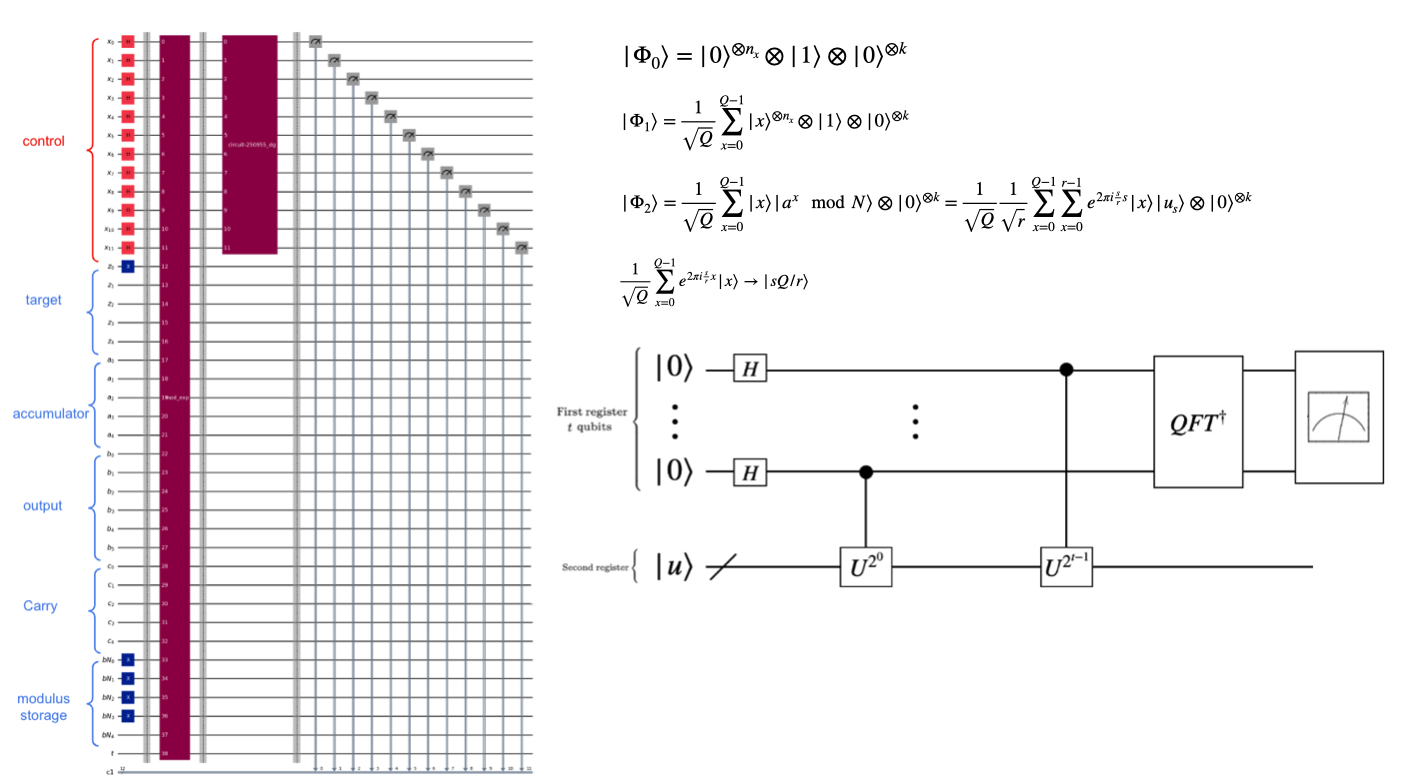
\includegraphics[scale=0.5]{images/Screenshot 2026-02-18 alle 20.50.34.png}
    \caption{Circuit diagram for Shor’s algorithm and generic QPE.}
\end{figure}

\section{4. Experimental Results}

\subsection{4.1 Measurement Outcomes and Period Recovery}

After applying the inverse QFT to the control register, the measurement histogram peaks at multiples of $2^{n_x}/r$. For example, in Fig. \ref{fig:histogram}
there is the case $N=33$, $a=7$,
the dominant measurement outcome is $m = 29491$ (binary: \texttt{111001100110011}),
giving $\varphi = 29491/32768 \approx 0.900$. The continued fraction expansion yields
the candidate $r=10$, which satisfies $7^{10} \equiv 1 \pmod{33}$. From this,
$\gcd(7^5-1,\, 33) = 3$ and $\gcd(7^5+1,\, 33) = 11$, correctly recovering the factors
$3 \times 11 = 33$.

\begin{figure}[h]
    \centering
    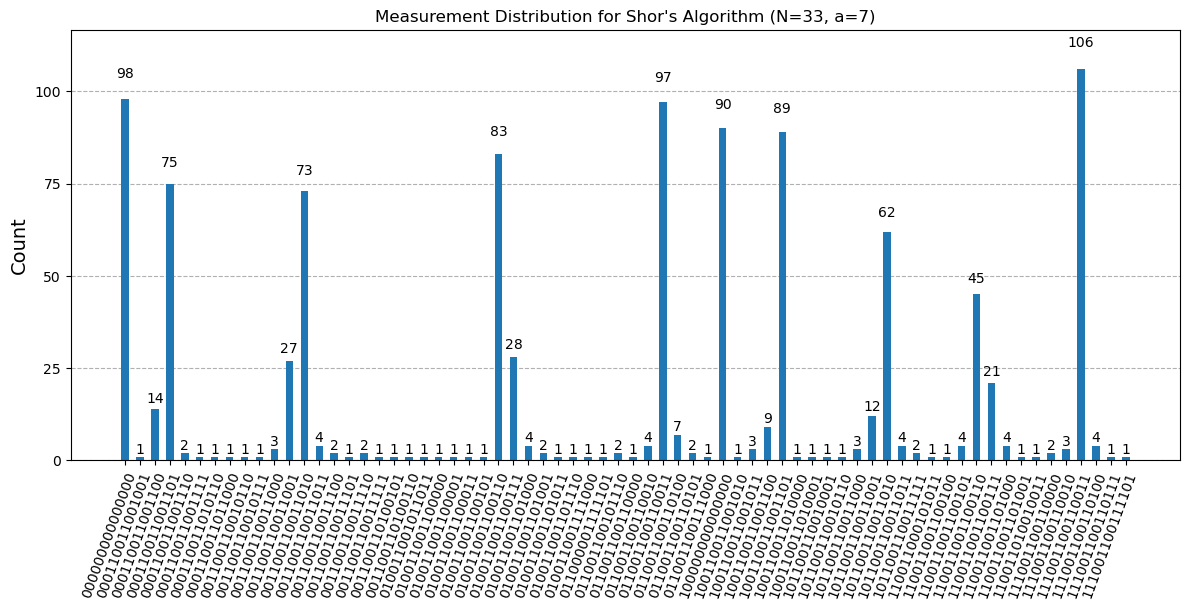
\includegraphics[width=0.65\textwidth]{images/c80f06a8-0760-4bef-afae-fc75092b38f4.png}
    \caption{Measurement distribution of the control register after applying the inverse
    QFT ($N=33$, $a=7$).}
    \label{fig:histogram}
\end{figure}

\subsection{4.2 Scalability}

Execution time was measured for $N \in \{15, 65, 133\}$ (corresponding to $L = 4, 7, 8$
bits). On a semi-log scale, the data lie close to the theoretical $\mathcal{O}(L^3)$
reference (Figure~\ref{fig:scaling}). 
The code was running in simulator MPS backend. 
The observed scaling is consistent with the theoretical polynomial growth of the algorithm's complexity.

\begin{figure}[h]
    \centering
    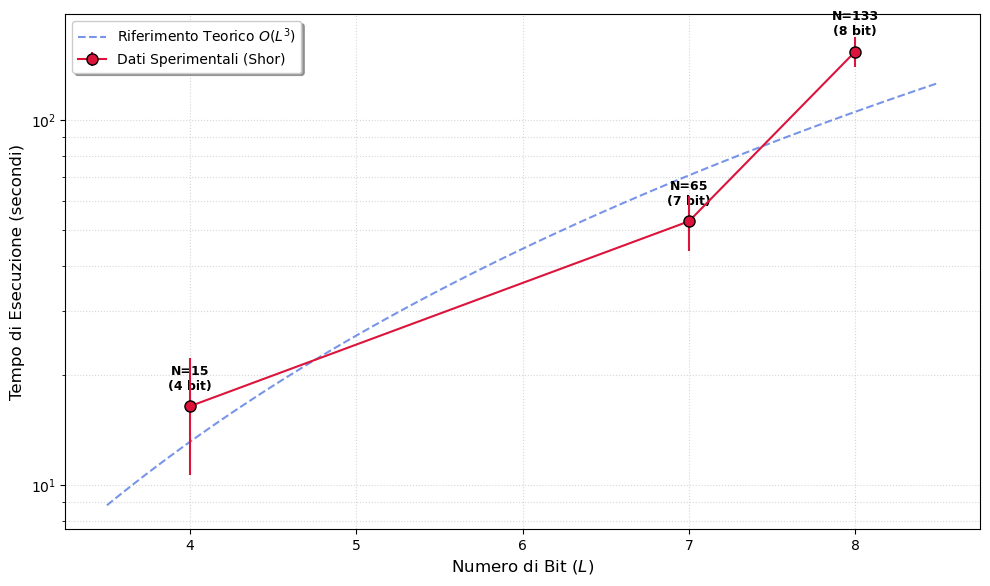
\includegraphics[width=0.65\textwidth]{images/034a5555-b9a0-49e0-8c5a-94f0cf4a48ae.png}
    \caption{Execution time vs.\ number of bits $L = \lceil\log_2 N\rceil$ on a
    semi-log scale. Are included 3 executions to estimate the error. Experiment was performed on MPS simulator backend.}
    \label{fig:scaling}
\end{figure}

\section{5. RSA Application}
One application of Shor's algorithm is the breaking of RSA, as it relies on the classical time limitations
of factoring the product of two large prime numbers.
To encrypt data the receiver chooses two large primes $p$ and $q$, 
computes $N = pq$ and $\phi(N) = (p-1)(q-1)$, then picks a public exponent $e$ coprime to $\phi(N)$.
Encryption and decryption are defined as
$c = m^e \bmod N$ and $m = c^d \bmod N$, with private key $d = e^{-1} \bmod \phi(N)$.
Shor's algorithm can be used to find the factors of $N$. Once $p$ and $q$ are known, $\phi(N)$ can be computed, and the private key $d$ can be derived from the public key $e$.


\section{References}
[1] Polynomial-Time Algorithms for Prime Factorization and Discrete Logarithms on a Quantum Computer, Peter W. Shor, 1997.

[2] Quantum Computation and Quantum Information, Michael A. Nielsen and Isaac L. Chuang, 2010.

[3] Quantum Networks for Elementary Arithmetic Operations, V. Vedral, A. Barenco, A. Ekert, 1996.

\end{document}